\section{MLP}
Yapay sinir ağları (ANN) ailesine ait bir modeldir. MLP, en az bir gizli katman içeren bir yapay sinir ağıdır ve en az bir giriş ve bir çıkış katmanı bulunur. Her katmandaki düğümler bir önceki katmandaki tüm düğümlerle bağlanır ve ağında içindeki bilgi akışını sağlar.

\begin{figure}[h]
    \centering
    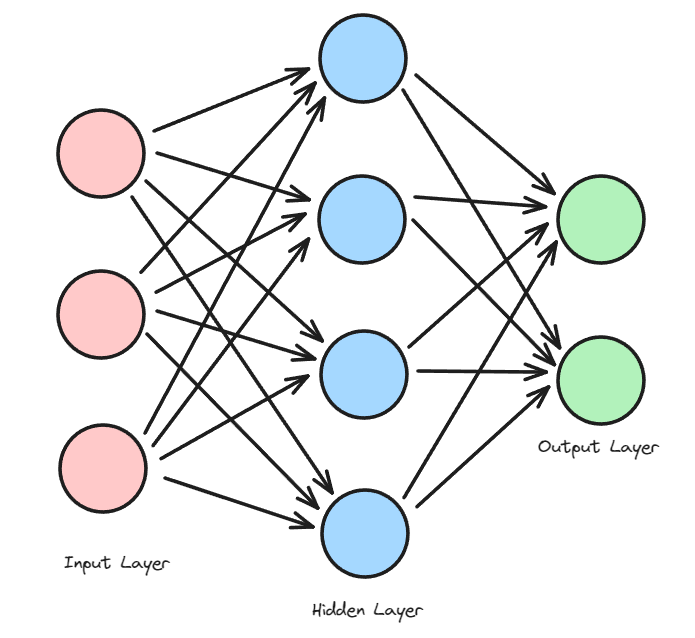
\includegraphics[width=1\textwidth]{images/mlp.png}
    \caption{Multi-layer perceptron.}
    \label{fig:enter-label}
\end{figure}

\subsection{Çalışma Adımları}
\begin{itemize}
    \item MLP modeli oluşturulur.
    \item Başlangıç ağırlıkları rastgele atanır.
    \item Giriş verisi her bir gizli katmandaki düğümler arasından çıkış katmanına doğru ilerler (forward propagation). Bu işlem, her bir katmandaki düğümlerde aktivasyon fonksiyonunun uygulanmasıyla gerçekleşir.
    \item İleri yayılma işleminden sonra tahmin edilen çıktılar ile gerçek değerler arasındaki hata hesaplanır.
    \item Hata hesaplamasından sonra geri yayılma (backward propagation) işlemi gerçekleştirilir. Geri yayılma, ağın içindeki hata miktarını geriye doğru hesaplar ve her bir ağırlığın bu hataya katkısını belirler.
    \item Gradyan iniş (gardient descent) ile geri yayılma işleminden elde edilen hata miktarına dayanarak, ağdaki ağırlıklar güncellenir.
    \item Belirli bir iterasyona kadar bu işlem tekrarlanır.
\end{itemize}

\subsection{Hiperparametreler}
\begin{table}[h]
\centering
{\scriptsize\renewcommand{\arraystretch}{0.4}
{\resizebox*{\linewidth}{0.4\textwidth}{
\begin{tabular}{|p{3cm}|p{2cm}|p{1cm}|p{5cm}|}
\hline
Parametre & Type & Default & Açıklama \\ \hline
hidden\_layer\_sizes & array-like & (100,) & Gizli katman sayısı. \\ \hline
activation & "identity", "logistic", "tanh", "relu" & "relu" & Aktivasyon fonksiyonu. \\ \hline
solver & "lbfgs", "sgd", "adam" & "adam" & Ağırlıkları güncellemek için kullanılan optimizasyon algoritması. \\ \hline
learning\_rate & "constant", "invscaling", "adaptive" & "constant" & Öğrenme oranı. \\ \hline
alpha & float & 0.0001 & Ağırlık düzenlemesi için kullanılır. \\ \hline
batch\_size & int & "auto" & Ağırlık güncellemesi sırasında kullanılan mini-batch sayısını belirler. \\ \hline
max\_iter & int & 20 & İterasyon sayısı. \\ \hline
\end{tabular}
}}}
\end{table}

\newpage